% !TeX program = lualatex
\documentclass{scrbook}
    
\usepackage[partial=upright]{unicode-math}
\usepackage{fontspec}
\usepackage{caption,subcaption}
\usepackage{graphicx}
\usepackage[main=ngerman,english]{babel}

\begin{document}
	\begin{figure}
		%
		\begin{subfigure}{0.5\linewidth}
			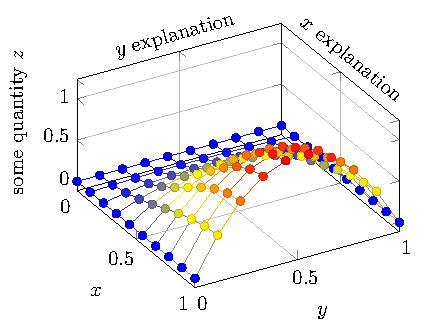
\includegraphics{3dplot_a.pdf}
		\end{subfigure}
		%
		\begin{subfigure}{0.5\linewidth}
			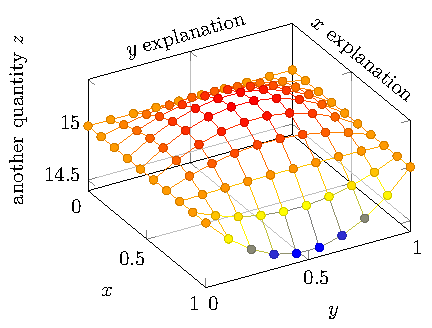
\includegraphics{3dplot_b.pdf}
		\end{subfigure}
		%
		\begin{subfigure}{0.5\linewidth}
			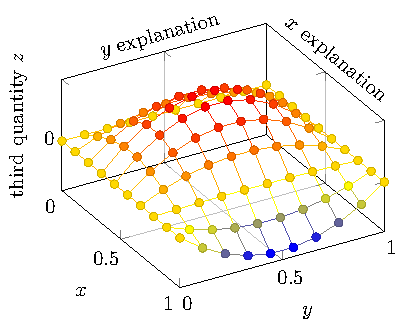
\includegraphics{3dplot_c.pdf}
		\end{subfigure}
		%
		\begin{subfigure}{0.5\linewidth}
			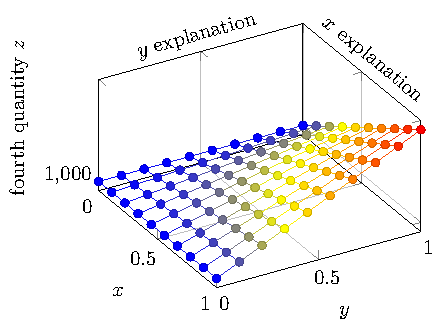
\includegraphics{3dplot_d.pdf}
		\end{subfigure}
		%
	\end{figure}
\end{document}

